\documentclass[conference]{IEEEtran}
\IEEEoverridecommandlockouts
% The preceding line is only needed to identify funding in the first footnote. If that is unneeded, please comment it out.
\usepackage{cite}
\usepackage{amsmath,amssymb,amsfonts}
\usepackage{algorithmic}
\usepackage{graphicx}
\usepackage{textcomp}
\usepackage{xcolor}
\def\BibTeX{{\rm B\kern-.05em{\sc i\kern-.025em b}\kern-.08em
    T\kern-.1667em\lower.7ex\hbox{E}\kern-.125emX}}

\setlength\arraycolsep{2pt}

\begin{document}

\title{State estimation, inertial measurement units, and legged robots\\
}

\author{\IEEEauthorblockN{1\textsuperscript{st} Ziegltrum}
\IEEEauthorblockA{\textit{Computer Science Department} \\
\textit{Stanford School of Engineering}\\
London, England \\
ziegltrum@gmail.com}
}

\maketitle

\begin{abstract}
Inertial measurement units have a long history of being used for state estimation. Unofortunately they accumulate error as they are used which can be mitigated by fusing another sensor's data, for instance with a Kalman filter. Legged robots often use IMUs to help estimate their state, in particular fusing leg odometry. The author proposes to study a dataset of a quadruped trotting, develop an EKF to estimate the quadruped's state from the IMU Data, compare it to the ground truth in the dataset, and then port the algorithm to a Raspberry Pi and an IMU Breakout board the author posseses.
\end{abstract}

\begin{IEEEkeywords}
state estimation, imu, quadruped
\end{IEEEkeywords}

\section{Literature Review}
\subsection{State Estimation and Inertial Measurement}
State estimation is a vital field of study for the control of dynamical systems. The inertial measurement unit, or IMU, is a sensor that has been widely used in state estimation.
Tazartes points out that an early example of a system using inertial measurement was the system used by the V2 rockets developed by Nazi Germany \cite{b1}. In the late 1940s and 50s, much research
was undergone and inertial navigation systems were used in fighter jets, before in 1968 the first inertial navigation system for commercial aircraft was certified \cite{b1}. Before the sensor was widely and cheaply available,
practitioners had to rely on other sensors. For example, in the problem of Satellite Rendezvous in 1960, Clohessy and Wiltshire suggested using a ground based radar system to track the initial satellite,
and a further infrared homing system to complete rendezvous \cite{b2}. H. Black in 1964 proposed a passive system using solar attitude detectors to determine the attitude of a satellite \cite{b3}.

One drawback to inertial measurement systems is their propensity to accumulate errors over time. If we have white noise in our x-axis linear acceleration estimate, we integrate to get to velocity and error grows quadratically. We integrate to get to position and error grows cubically. One study in 1973 found that 45 minute flights using a three-axis inertial measurement system accumulated errors of $\pm 2^{\circ}$ \cite{b4}. Over longer periods of time this error can accumulate even more significantly. In 1966, Friedlander proposed using the Kalman filter to fuse celestial sensors with inertial measurement, "significantly reducing the long term effects of inertial gyro and accelerometer errors" \cite{b5}.

Fast forward to today and Micro-Electro-Mechanical Systems (MEMS) IMUs are cheaper, more compact, and require less processing power than earlier IMUs, leading to widespread usage \cite{b6}. In robotics, we often see applications fusing IMU data with other sensors to solve for IMU drift error and synergize with other sensors. For example, in visual-inertial odometry (VIO) the state including pose and velocity of an agent is estimated using the input of camera and IMU which are both cheap sensors \cite{b7}. Landmarks from the camera can be used to estimate state and fused with estimates from the IMU (loosely-coupled) or IMU measurements can be used to predict location of features (tightly-coupled) often using the extended Kalman filter \cite{b7}. Another example is lidar inertial odometry, where IMU data is fused with Lidar data, de-skewing it, and features from the Lidar are used to estimate poses \cite{b8}. A commonality in VIO and lidar inertial odometry is that both approaches take advantage of the high update rate of the IMU and that measurements don't depend on the surrounding scene, fusing it with other sensors that may not have those characteristics but have other characteristics that mitigate IMU weak-points like tendency to accumulate drift \cite{b7} \cite{b8}.

\subsection{Legged Robots and State Estimation}
Legged robots pose advantages and disadvantages in comparison to wheeled or tracked robots. Legged robots may be able to navigate complex non-planar terrain that would stump wheeled robots, like stairs. For example, in the late 1970s the legged spider-like robot KUMO-I was the world's first success in sensor-based stair climbing \cite{b9}. On the flip side legged robots may be more complex to control than wheeled robots. To get a robot using differential drive to move forward we run both wheels forward. To get a quadruped with 3 joints per leg moving forward we need to model the inverse kinematics of each foot to understand the relationship between all of the joint angles and the end effector position. Then we need to apply a walking gait that manages the trade-offs between stability and speed to coordinate the foot movement and move the quadruped forward.

One of the first autonomous legged robots in the United States was the University of Southern California's phony pony, in the late 1960s \cite{b9}. This robot had two joints per leg and used flip flop digital logic to produce several gait patterns \cite{b9}. These flip flop circuits could store state information and thusly the robot could autonomously walk. Moving to the modern era, robots such as BigDog balance moving at human-walking speeds using the sensed behavior of the legs combined with inertial sensors \cite{b10}.

Looking into this fusion, the Anymal robot also fuses IMU, leg kinematics, and ground contact measurements and specifically it uses a framework proposed by Bloesch et al \cite{b11}. This framework differentiates itself from other state estimation frameworks discussed earlier in this paper like VIO or lidar inertial odometry by taking into account that legged robots interact with intermittent ground contact from end effectors \cite{b12}. It uses "an Observability Constrained Extended Kalman Filter that fuses kinematic encoder data with on-board IMU measurements" \cite{b12}.  However, the authors point out in an observability analysis that "typical operating points can lie very close to singular cases," and this can cause bad convergence quality, suggesting an implementation that doesn't estimate accelerometer and gyroscope biases \cite{b12}. Another interesting model for state estimation of quadrupeds using joint encoders, torque sensors, and IMU, that produces high-frequency, smooth, attitude and velocity estimates is given in \cite{b13}. The authors use a non-linear attitude observer, leg odometry, and fuse the two using a Kalman filter \cite{b13}. 

 Another example of an innovative approach is given in this study \cite{b15} where the authors use factor graph optimization to tightly fuse and smooth inertial navigation, leg odometry, and visual odometry. The authors exploit smoothing approaches applied to Visual Inertial Navigation Systems to fuse this with legged odometry\cite{b15}. Other innovative approaches to state estimation for legged robots include learning-based approaches. For instance, in one study a state estimator using convolutional neural networks on displacement measurement from IMU data was proposed \cite{b14}. The authors use the learned displacement measurement from IMU data and fuse it with leg odometry, offering 	benefits in environments where leg odometry is unreliable like terrains with slippage \cite{b14}.

\subsection{Summary}
As we have seen, IMUs are an important sensor in state estimation and in state estimation for legged robots. IMUs have some drawbacks in terms of drift, but this can be mitigated by fusing with other sensor data \cite{b5} \cite{b7} \cite{b12}. Particular to legged robots, many approaches have been suggested that fuse IMU data with leg odometry data \cite{b12} \cite{b13} \cite{b15}. In summary, legged robots have potential, are exciting to study, and IMUs are often an integral part of state estimation for legged robots.

\section{Project Proposal}
This paper focuses focus on the use of inertial measurement units for orientation estimation. One interesting dataset containing IMU data from an accelerometer, a magnetometer, and a gyroscope is found \cite{b20}. An EKF is developped to estimate the orientation of the system. From here the ground truth data from the dataset is compared to the measurement as well as to the estimate from the EKF.

\section{Problem Setup}

How do we take a nine degree of freedom inertial measurement unit, including an accelerometer, a gyroscope, and a magnetometer, and use this to get position, velocity, and orientation? Traditional methods of double integrating linear angular acceleration to get to orientation accumulate drift and error over time. We will use an approach similar to \cite{b19} that uses the gravity vector in tandem with the earth's magnetic field vector to obtain static state estimates of orientation. This avoid drift accumulation in the orientation estimate. We can also avoid errors by fusing the output of the gyroscope measurements and the orientation estimate from the digital compass to get a better estimate than relying on just one method.

\section{Methods}

\subsection{Orientation}

We have outputs of $a_{acc}$ from the accelerometer measuring linear acceleration, $H_{mag}$ from the magnetometer measuring the Earth's magnetic field, and $\omega_{gyro}$ angular acceleration from the gyroscope. We will obtain orientation from the accelerometer's x and y data, in combination with the magnetometer data, assuming little to no angular or linear acceleration. We will also get an orientation estimate from the double integral of angular acceleration, and a position estimate from the double integral of linear acceleration. We will fuse this all together in an extended Kalman filter to get better estimates than we could for just one of the methods as per Fig \ref{fig:ekf}.

\begin{figure}[h!]
  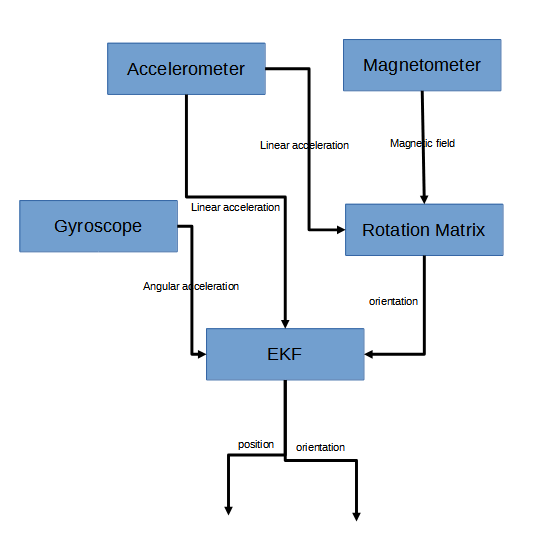
\includegraphics[width=\columnwidth]{fig_2_ekf.png}
  \caption{Sensors and EKF System}
  \label{fig:ekf}
\end{figure}


Let's use Euler angle formulations with y rotation, roll ($\phi$), x rotation, pitch ($\theta$), and z rotation, yaw ($\psi$), and for estimation of position and velocity we will use a similar method to \cite{b18}. We define gravity as per \eqref{eq:grav} where g represents the gravitational constant, and we define magnetic vector of earth as per \eqref{eq:magn} where a and b are components of earth's magnetic vector in the world frame.

\begin{align}
g_w =& \begin{bmatrix}0& 0& -g\end{bmatrix}^T \label{eq:grav} \\
H_w =& \begin{bmatrix}a& 0& b\end{bmatrix}^T \label{eq:magn}
\end{align}


Similar to \cite{b19} gravity of the world frame relates to gravity in the body frame as per \eqref{eq:grav_body_to_world}, where $R_{w}^b$ denotes rotation matrix from world to the body frame. The rotation matrix from world to the body frame can be defined in \eqref{eq:rotation_world_body}, where c represents cos() and s represents sin(). This expresses a rotation of pitch, then roll, then yaw, or x, y, z, where the order matters.

\begin{align}
g_w =& R_{b}^w g_b \label{eq:grav_body_to_world} \\
(R_{w}^b) =& \begin{bmatrix} c\theta c\psi& c\theta s\psi& -s\theta\\
					  s \phi s\theta c\psi - c \phi s\psi& s\phi s\theta s\psi + c\phi c\psi& s \phi c \theta\\
					 c \phi s \theta c \psi + s \phi s \psi& c \phi s \theta s\psi - s \phi c\psi& c \phi c \theta	\end{bmatrix}\label{eq:rotation_world_body}
\end{align} 

The accelerometer gives us gravitational accelerations in the robot body reference frame. We can relate the robot body gravitational acceleration to the world acceleration via \eqref{eq:gravity_world_to_body}, assuming the body is in a steady state with respect to acceleration.
\begin{align}
g_b =& R_w^b g_w, \text{where } R_w^b = (R_b^w)^T\\
g_b =& \begin{bmatrix} g_{bx}\\ g_{by}\\ g_{bz} \end{bmatrix} = R_{w}^b g_w = R_{wb} (-g) = (-g) \begin{bmatrix} -sin \theta \\ sin \phi cos \theta \\ cos \phi cos \theta \end{bmatrix} \label{eq:gravity_world_to_body}
\end{align}

We can calculate $\phi$ and $\theta$ as per Fig \ref{fig:pitch}, with reference only to earth's gravitational vector avoiding accumulation and drift errors, but assuming litttle to no acceleration apart from gravity as per \cite{b19}.
\begin{align}
\phi =& arctan \left( \frac{g_{by}}{g_{bz}} \right)\\
\theta =& arctan \left( \frac{ - g_{bx}}{\sqrt{g_{by}^2 + g_{bz}^2}} \right ) \nonumber \\
\theta =& arctan \left( \frac{ - g_{bx}}{(g_{by} sin \phi + g_{bz} cos\phi} \right ) 
\end{align}

\begin{figure}[h!]
  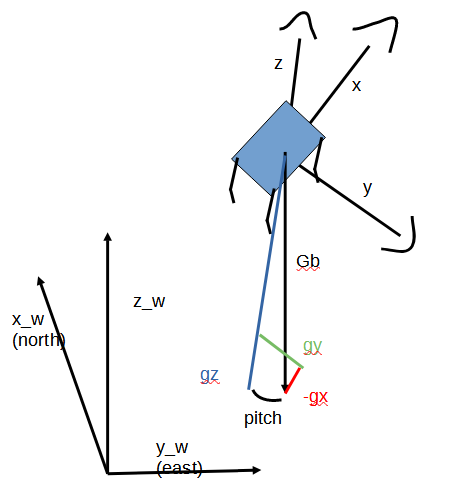
\includegraphics[width=\columnwidth]{fig_1_pitch.png}
  \caption{World Frame vs Robot Frame}
  \label{fig:pitch}
\end{figure}

With regards to yaw, we will use the three components of earth's magnetic field vector and transform the main plane of the magnetometer into the horizontal plane in the world frame using roll and pitch. Then we can calculate yaw, using \eqref{eq:yaw}, because after applying pitch and roll, yaw is all that is left.

\begin{align}
H^{hor} =& \begin{bmatrix} H_x^{hor}& H_y^{hor}& H_{z}^{hor}\end{bmatrix}^T = R(y, \theta) R(x, \phi) H^w \nonumber \\
R_w^b =& R(z, \psi) R(y, \theta) R(x, \phi)\\
\psi =& arctan(H_y^{hor} / H_x^{hor})\label{eq:yaw}
\end{align}

We've solved for the orientation without using integration and accumulating errors and drift. That said, this assumes zero or small rotation and translational acceleration so we isolate acceleration to just gravity.

\subsection{State Model and Dynamics}

Similar to \cite{b19} we define acceleration as the sensor measurement as the sum of gravity, and the rotational and linear acceleration.

\begin{align}
\begin{bmatrix} a_x^b\\ a_y^b\\ a_y^b\end{bmatrix} = \begin{bmatrix} acc_x^b - \omega_y^b V_y^b + g sin \theta\\
													  acc_x^b + \omega_x^b V_z^b - \omega_z^b V_x^b - g sin \phi cos \theta \\
													  acc_x^b - \omega_x^b V_y^b + \omega_y^b V_x^b - g cos \phi cos \theta\end{bmatrix}
\end{align}

Position and velocity in discrete time:
\begin{align}
V_{b_{t+1}} = V_{b_{t}} + a_{bt} \delta t\\
S_{b_{t+1}} = S_{b_{t}} + V_{bt} \delta t
\end{align}

Angular rates
\begin{align}
\begin{bmatrix} \omega_x^b\\ \omega_y^b\\ \omega_z^b \end{bmatrix} =& \begin{bmatrix} \omega_x^w\\ 0\\ 0\end{bmatrix} + R^T(x, \phi) \begin{bmatrix} 0\\ \omega_x^w\\ 0\end{bmatrix} \\
& + R^T(x, \phi) R^T(y, \theta) \begin{bmatrix} 0\\ 0\\ \omega_x^w \end{bmatrix} \\
\begin{bmatrix} \omega_x^w\\ \omega_y^w\\ \omega_z^w \end{bmatrix} =& R_b^{'w} (\theta) \omega^b\\
=& \begin{bmatrix} 1& sin\phi tan\theta& cos\phi tan\theta\\
			     0& cos \phi& -sin\phi\\
			    0& sin\phi / cos \theta& cos\phi/cos\theta \end{bmatrix} \begin{bmatrix} \omega_x^b\\ \omega_y^b\\ \omega_z^b \end{bmatrix}  \label{angular_rates_world_eq}
\end{align}

\begin{align}
\begin{bmatrix} S^w\\ V^b\\ \theta^w \end{bmatrix}_{t+1} = \begin{bmatrix} S_t^w + R_b^w (\theta) (V_t^b \delta t) \\
														      V_t^b + \delta T (a_t - \vec{g} - \vec{\omega} x \vec{v})_t \\
														      \theta_t^w + R^{'w}_b (\theta) \omega_t^b \end{bmatrix}
\end{align}

State matrix only looking at the orientation. Hopefully more correct.
\begin{align}
\begin{bmatrix} 
\theta_{t}^{w}\end{bmatrix} =& \begin{bmatrix} 
\theta_{t-1}^{w} + \delta t R_b^{\prime w}(\theta_{t-1}) \omega_{t-1}^b \end{bmatrix} \nonumber
\end{align}

Substituting equation \ref{angular_rates_world_eq} for the rotation from body to world, and doing the matrix multiplication with the angular velocities in body frame.
\begin{align}
\begin{bmatrix} 
\theta_{x_{t}}^{w}\\
\theta_{y_{t}}^{w}\\
\theta_{z_{t}}^{w}\end{bmatrix} =& \begin{bmatrix} 
\theta_{x_{t-1}}^{w} + \delta t (\omega_{x_{t-1}}^b + sin\phi tan \theta \omega_{y_{t-1}}^b + cos\phi tan\theta \omega_{z_{t-1}}^b) \\
\theta_{y_{t-1}}^{w} + \delta t (cos\phi \omega_{y_{t-1}}^b - sin\phi \omega_{z_{t-1}}^b) \\
\theta_{z_{t-1}}^{w} + \delta t (sin\phi  \omega_{y_{t-1}}^b / cos \theta + cos\phi \omega_{z_{t-1}}^b  / cos\theta) \end{bmatrix} \nonumber
\end{align}

This is non-linear, so we will take the jacobian, the derivative with respect to each element of the state matrix, and use an extended kalman filter. A will be 3x3, where ith row looks at the equation for ith element of state matrix, and each jth column is derivative of ith equation element with respect to jth element in state matrix.

\begin{align*}
\phi =  \theta_{x_{t}}^{w}, \theta =&  \theta_{y_{t}}^{w}, \psi =  \theta_{z_{t}}^{w}\\
A[0][0] =& \frac{\partial \theta_{x_{t}}^{w}}{\partial \theta_{x_{t}}^{w}}\\
A[0][0] =& 1 + cos\phi tan\theta \omega_{y_{t-1}}^b - sin\phi tan\theta  \omega_{z_{t-1}}^b \\
A[0][1] =& \frac{\partial \theta_{x_{t}}^{w}}{\partial \theta_{y_{t}}^{w}}\\
A[0][1] =& sin\phi (\frac{1}{tan\theta})^2 \omega_{y_{t-1}}^b +  cos\phi (\frac{1}{tan\theta})^2  \omega_{z_{t-1}}^b \\
A[0][2] =& \frac{\partial \theta_{x_{t}}^{w}}{\partial \theta_{z_{t}}^{w}}\\
A[0][2] =& 0 \\
A[1][0] =& \frac{\partial \theta_{y_{t}}^{w}}{\partial \theta_{x_{t}}^{w}}\\
A[1][0] =& -sin\phi \omega_{y_{t-1}}^b -cos\phi \omega_{z_{t-1}}^b  \\
A[1][1] =& \frac{\partial \theta_{y_{t}}^{w}}{\partial \theta_{y_{t}}^{w}}\\
A[1][1] =& 1  \\
A[1][2] =& \frac{\partial \theta_{y_{t}}^{w}}{\partial \theta_{z_{t}}^{w}}\\
A[1][2] =& 0\\
A[2][0] =& \frac{\partial \theta_{z_{t}}^{w}}{\partial \theta_{x_{t}}^{w}}\\
A[2][0] =& cos\phi \omega_{y_{t-1}}^b / cos \theta - sin\phi \omega_{z_{t-1}}^b / cos\theta \\
A[2][1] =& \frac{\partial \theta_{z_{t}}^{w}}{\partial \theta_{y_{t}}^{w}}\\
A[2][1] =& sin\phi \omega_{y_{t-1}}^b (\frac{-1}{cos^2 \theta})(-sin\theta)  + cos\phi \omega_{z_{t-1}}^b (\frac{-1}{cos^2 \theta})(-sin\theta) \\
A[2][2] =& \frac{\partial \theta_{z_{t}}^{w}}{\partial \theta_{z_{t}}^{w}}\\
A[2][2] =& 1 \\
\end{align*}




For the measurement model, let's assume static state. We could flesh this out further by making our acceleration measurement equal to linear, rotational, and gravity vector. But let's keep it simple for now. In the below, we model measurements of yaw from magnetometer calculation, and accelerometer observations.
\begin{align}
y_t(\theta) = \begin{bmatrix} \psi_m \\ a_x^b \\  a_y^b \\  a_z^b \end{bmatrix} =& \begin{bmatrix} \psi\\
															 -g -sin \theta\\
													              -g sin \phi cos \theta \\
													               -g cos \phi cos \theta \end{bmatrix} \nonumber
\end{align}

\begin{align*}
\theta_{x_{t}}=&\phi, \theta_{y_{t}}=\theta, \theta_{z_{t}}=\psi \\
C[0][0] =& \frac{\partial y_t(\theta)}{\partial\theta_{x_{t}}}\\
C[0][0] = & 0 \\
C[0][1] = & -g (-cos\theta) \\
C[0][2] = & 0 \\
C[1][0] = & -g cos\theta cos\phi \\
C[1][1] = & -g sin\phi(-sin\theta)\\
C[1][2] = & 0\\
C[2][0] = & -g (-sin\phi) cos\theta\\
C[2][1] = & -g cos\phi (-sin\theta)\\
C[2][2] = & 0\\
\end{align*}


To get expected measurement:
\begin{align}
\begin{bmatrix} \phi \\ \theta \\ \psi \end{bmatrix} =& \begin{bmatrix} arctan( g_y^b / g_z^b )\\
													arctan( - g_x^b / (g_y^b sin\phi + g_z^b cos\phi))\\
													arctan((m_y^b cos\theta - m_z^b sin\theta)  / \\
\quad - (M_x^b cos\theta + M_z^b sin\theta))
\end{bmatrix} \nonumber
\end{align}



\section{Results}

The results showed that the model does not fit well, and was not implemented well. In particular the sensor measurement model, given the IMU data, did not track well to the ground truth given in the dataset as per Fig \ref{fig:true_orientation}.  This establishes that there were problems early on.
\begin{figure}[h!]
  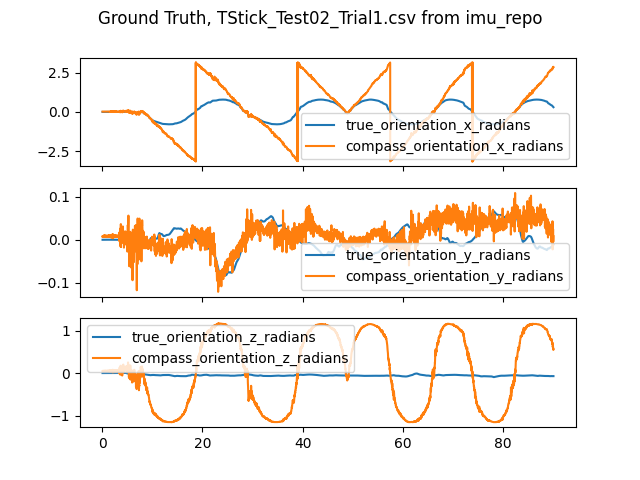
\includegraphics[width=\columnwidth]{true_values_vs_measurements.png}
  \caption{True Orientation vs Digital Compass Estimate}
  \label{fig:true_orientation}
\end{figure}

Furthermore, though the dataset used from \cite{b20} only had ground truth for orientation of the robot, a 9 DOF state model was used. This introduced complexity, especially in the derivation of the dynamics and the measurement models which could have introduced error into the system.  One row of the A matrix is given as an example. The sensor model with nested trigonometric functions proved a similar challenge.

\begin{align*}
A_{0,0} =& 1, A_{0,1} = 0, A_{0,2} = 0\\
A_{0,3} =& \delta t cos \theta cos \psi \\
A_{0,4} =& \delta t cos \theta sin \psi \\
A_{0,5} =&  \delta t sin \theta, A_{0,6} =  0 \\
A_{0,7} =& (V_x^b (-sin \theta) cos \psi + V_y^b (-sin \theta) sin \psi - V_z^b cos \theta) \delta t \\
A_{0,8} =& \delta t (V_x^b cos \theta (-sin \psi ) + V_y^b cos \theta cos \psi)\\
\end{align*}

\begin{figure}[h!]
  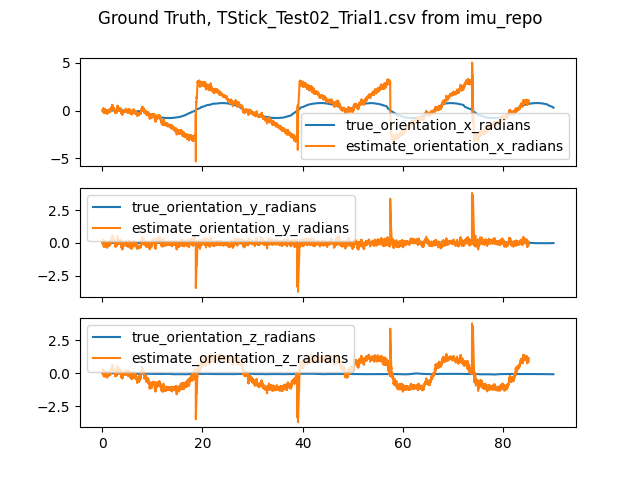
\includegraphics[width=\columnwidth]{true_values_vs_estimates.png}
  \caption{True Orientation vs EKF Estimate}
  \label{fig:orientation_estimate}
\end{figure}

In particular, the estimate of orientation from the EKF model does not track the actual trajectory from the dataset as per Fig \ref{fig:orientation_estimate}.

Unfortunately the poor tracking is not noted in the variance. The variance of the system does not blow up, though the system does not track as per Fig \ref{fig:variance}.
\begin{figure}[h!]
  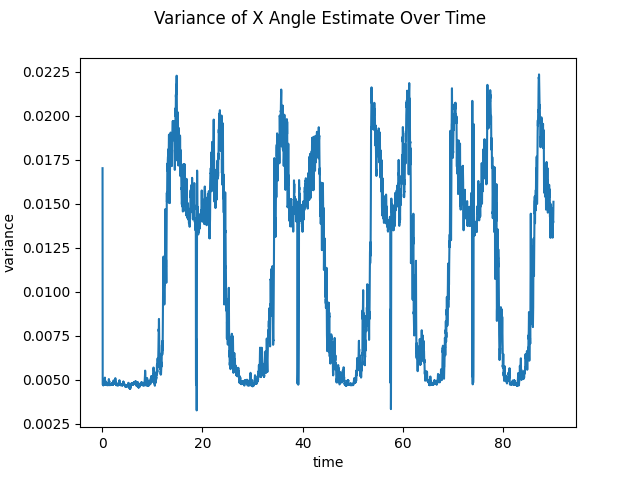
\includegraphics[width=\columnwidth]{variance_over_time.png}
  \caption{Variance of X Angle}
  \label{fig:variance}
\end{figure}


\subsection{Lessons Learned and Next Steps}

The authors learned some valuable lessons from this project. In particular, to start with easier scenarios and build up to more complex ones. Simplifying the states in this estimation problem could have made it more approachable. Also, using a simpler simulation instead of live data may have also helped.

In terms of next steps, after submitting this report the author intends to revist IMUs and spend more time on the measurement model and the state model to get a better system. Working in 3 dimensions and with real data is challenging, but rewarding.


\begin{thebibliography}{00}
\bibitem{b1} D. Tazartes, (2014). ``An historical perspective on inertial navigation systems,`` 1-5. 10.1109/ISISS.2014.6782505. 
\bibitem{b2} W.H. Clohessy, R.S. WILTSHIRE, ``Terminal guidance system for satellite rendezvous,`` J.Aerosp. Sci. 27 (9) (1960) 653–658, http://dx.doi.org/10.2514/8.8704.
\bibitem{b3} H.D. Black, ``A passive system for determining the attitude of a satellite,`` AIAA Journal 1964 2:7, 1350-1351
\bibitem{b4} Wolf, Thomas D., and Robert C. McCracken. ``Ground and flight experience with a strapdown inertial measuring unit and a general purpose airborne digital computer,`` No. H-735. 1973.
\bibitem{b5} Friedlander, Alan L. ``Analysis of an optimal celestial-inertial navigation concept for low-thrust interplanetary vehicles,`` No. NASA-CR-457. 1966.
\bibitem{b6} Ahmad, Norhafizan, Ghazilla, Raja Ariffin Raja, and Khairi, Nazirah M. ``Reviews on various inertial measurement unit (IMU) sensor applications,`` International Journal of Signal Processing Systems 1.2 (2013): 256-262.
\bibitem{b7} Scaramuzza, Davide, and Zichao Zhang. ``Visual-inertial odometry of aerial robots,`` arXiv preprint arXiv:1906.03289 (2019).
\bibitem{b8} H. Ye, Y. Chen and M. Liu, ``Tightly Coupled 3D Lidar Inertial Odometry and Mapping,`` 2019 International Conference on Robotics and Automation (ICRA), Montreal, QC, Canada, 2019, pp. 3144-3150, doi: 10.1109/ICRA.2019.8793511.
\bibitem{b9} Priyaranjan Biswal, Prases K. Mohanty, ``Development of quadruped walking robots: A review,`` Ain Shams Engineering Journal, Volume 12, Issue 2, 2021
\bibitem{b10} Raibert, Marc, et al. ``Bigdog, the rough-terrain quadruped robot.`` IFAC Proceedings Volumes 41.2 (2008): 10822-10825.
\bibitem{b11} Hutter, Marco, et al. ``Anymal-a highly mobile and dynamic quadrupedal robot.`` 2016 IEEE/RSJ international conference on intelligent robots and systems (IROS). IEEE, 2016.
\bibitem{b12} Bloesch, Michael, et al. ``State estimation for legged robots-consistent fusion of leg kinematics and IMU.`` Robotics 17 (2013): 17-24.
\bibitem{b13} Fink, Geoff, and Claudio Semini. ``Proprioceptive sensor fusion for quadruped robot state estimation.`` 2020 IEEE/RSJ International Conference on Intelligent Robots and Systems (IROS). IEEE, 2020.
\bibitem{b14} Buchanan, Russell, et al. ``Learning inertial odometry for dynamic legged robot state estimation.`` Conference on Robot Learning. PMLR, 2022.
\bibitem{b15} Wisth, David, Marco Camurri, and Maurice Fallon. ``Robust legged robot state estimation using factor graph optimization.`` IEEE Robotics and Automation Letters 4.4 (2019): 4507-4514.
\bibitem{b16} G. Fink and C. Semini, ``Proprioceptive Sensor Dataset for Quadruped Robots,`` IEEE Dataport, 2019, DOI:10.21227/4vxz-xw05
\bibitem{b17} G. Fink and C. Semini, (2019), ``Propioceptive Sensor Dataset for Quadrupeds,`` at the workshop on Visual-Inertial Navigation: Challenges and Applications in the IEEE/RSJ Internation Conference on Intelligent Robots and Systems (IROS), Macau, China, Nov. 2019, pp. 1–5
\bibitem{b18} Alatise, Mary B., and Gerhard P. Hancke. ``Pose estimation of a mobile robot based on fusion of IMU data and vision data using an extended Kalman filter`` Sensors 17.10 (2017): 2164.
\bibitem{b19} Zhao, He, and Zheyao Wang. ``Motion measurement using inertial sensors, ultrasonic sensors, and magnetometers with extended kalman filter for data fusion.`` IEEE Sensors Journal 12.5 (2011): 943-953.
\bibitem{b20} Szczesna, Agnieszka and Skurowski, Przemysław and Pruszowski, Przemyslaw and Peszor, Damian and Paszkuta, Marcin and Wojciechowski, Konrad. (2016). Reference Data Set for Accuracy Evaluation of Orientation Estimation Algorithms for Inertial Motion Capture Systems.
\end{thebibliography}

On implementing this algorithm on a real IMU, if the author runs out of time or this makes the scope too big, this could get cut. But, the author has worked extensively with Raspberry Pi's before and would like to look at a real life IMU. The author already posseses a Raspberry Pi 3b+ and an IMU breakout board (based on BNO085). The author proposes to create a docker container that can interface with the IMU and produce a dataset of measurements and estimations, using the algorithm developed earlier. Then the author could conduct a single experiment moving the imu to a known location over a known period of time, and comparing the estimate produced to the expected end position.

One risk of the project is related to project scope. The author is working alone, therefore the decision to focus on IMU data exclusively. With this focus, the author has a better chance of delivering a successful project, including the real life component using the IMU breakout board.

\begin{align*}
A_{0,0} =& 1\\
A_{0,1} =& 0\\
A_{0,2} =& 0\\
A_{0,3} =& \delta t cos \theta cos \psi \\
A_{0,4} =& \delta t cos \theta sin \psi \\
A_{0,5} =&  \delta t sin \theta \\
A_{0,6} =&  0 \\
A_{0,7} =& (V_x^b (-sin \theta) cos \psi + V_y^b (-sin \theta) sin \psi - V_z^b cos \theta) \delta t \\
A_{0,8} =& \delta t (V_x^b cos \theta (-sin \psi ) + V_y^b cos \theta cos \psi)\\
A_{1,0} =& 0\\
A_{1,1} =& 1\\
A_{1,2} =& 0\\
A_{1,3} =& \delta t ( s \phi s\theta c\psi - c \phi s\psi)  \\
A_{1,4} =& \delta t  (s\phi s\theta s\psi + c\phi c\psi) \\
A_{1,5} =&  \delta t (s \phi c \theta) \\
A_{1,6} =&  \delta t (V_x^b (c\phi s \theta c \psi +s\phi s\psi) + V_y^b (c\phi s \theta s \psi -s\phi c\psi) + V_z^b(c \phi c \theta)) \\
A_{1,7} =&   \delta t (V_x^b(c\phi cos \theta c \psi) + V_y^b(s \phi cos \theta s \psi) + V_z^b(s \phi ( -s \theta)))\\
A_{1,8} =& \delta t (V_x^b(s\phi s\theta (-s\psi)) + V_y^b(s \phi s \theta c \psi + c\phi (-s\psi)))\\
A_{2,0} =& 0\\
A_{2,1} =& 0\\
A_{2,2} =& 1\\
A_{2,3} =& \delta t  (c \phi s \theta c \psi + s \phi s \psi)   \\
A_{2,4} =& \delta t ( c \phi s \theta s\psi - s \phi c\psi) \\
A_{2,5} =&  \delta t (c \phi c \theta) \\
A_{2,6} =&  \delta t (V_x^b ((-s \phi)s\theta c \psi + c \phi s \psi) + V_y^b ((-s \phi) s \theta s \psi - c \phi c \psi) + V_z^b((-s \phi) c \theta)) \\
A_{2,7} =&   \delta t (V_x^b(c\phi c\theta c\psi) + V_y^b(c\phi c\theta s\psi) + V_z^b((c \phi (-s \theta))))\\
A_{2,8} =& \delta t (V_x^b(c\phi s \theta (-s\psi) +s\phi c \psi) + V_y^b(c \phi s \theta c \psi + s \phi s \psi))\\
\end{align*}

\begin{align*}
A_{3,0} =& 0\\
A_{3,1} =& 0\\
A_{3,2} =& 0\\
A_{3,3} =& 1 \\
A_{3,4} =& \delta T (-\omega_z^b) \\
A_{3,5} =& \delta T (\omega_y^b) \\
A_{3,6} =& 0 \\
A_{3,7} =& \delta T (-g cos \theta) \\
A_{3,8} =& 0\\
A_{4,0} =& 0\\
A_{4,1} =& 0\\
A_{4,2} =& 0\\
A_{4,3} =& \delta T (\omega_z^b) \\
A_{4,4} =& 1 \\
A_{4,5} =&  \delta T (-\omega_x^b) \\
A_{4,6} =& \delta T(g cos \phi cos \theta)\\
A_{4,7} =& \delta T (g sin \phi (-sin \theta) \\
A_{4,8} =& 0 \\
A_{5,0} =& 0\\
A_{5,1} =& 0\\
A_{5,2} =& 0\\
A_{5,3} =& \delta T (-\omega_y^b) \\
A_{5,4} =& \delta T (\omega_x^b) \\
A_{5,5} =&  1 \\
A_{5,6} =& \delta T(g (-sin \phi) cos \theta)\\
A_{5,7} =& \delta T (g cos \phi (-sin \theta) \\
A_{5,8} =& 0 \\
\end{align*}

\begin{align*}
A_{6,0} =& 0\\
A_{6,1} =& 0\\
A_{6,2} =& 0\\
A_{6,3} =& 0 \\
A_{6,4} =& 0 \\
A_{6,5} =& 0 \\
A_{6,6} =& 1 + cos \phi tan \theta \omega_y^b - sin \phi tan \theta \omega_z^b \\
A_{6,7} =& sin\phi sec^2 \theta \omega_y^b +cos \phi sec^2 \theta \omega_z^b\\
A_{6,8} =& 0 \\
A_{7,0} =& 0\\
A_{7,1} =& 0\\
A_{7,2} =& 0\\
A_{7,3} =& 0 \\
A_{7,4} =& 0 \\
A_{7,5} =& 0 \\
A_{7,6} =& -sin\phi \omega_y^b - cos \phi \omega_z^b \\
A_{7,7} =& 1\\
A_{7,8} =& 0\\
A_{8,0} =& 0\\
A_{8,1} =& 0\\
A_{8,2} =& 0\\
A_{8,3} =& 0 \\
A_{8,4} =& 0 \\
A_{8,5} =& 0 \\
A_{8,6} =& (cos \phi / cos \theta) \omega_y^b + (-sin\phi / cos\theta) \omega_z^b \\
A_{8,7} =& sin \phi \omega_y^b (-1 / ( cos \theta )^2) (-sin \theta) + cos \phi \omega_z^b (-1/(cos \theta)^2 (-sin \theta) \\
A_{8,8} =& 1\\
\end{align*}

C will be a 3x9 matrix.
\begin{align*}
C_{0,0} =& 0\\
C_{0,1} =& 0\\
C_{0,2} =& 0\\
C_{0,3} =& 0 \\
C_{0,4} =& 0 \\
C_{0,5} =& 0 \\
C_{0,6} =& 1 \\
C_{0,7} =& 0 \\
C_{0,8} =& 0\\
C_{1,0} =& 0\\
C_{1,1} =& 0\\
C_{1,2} =& 0\\
C_{1,3} =& 0 \\
C_{1,4} =& 0 \\
C_{1,5} =& 0 \\
C_{1,6} =& 2 cos(\phi) cos(\theta) / (cos(2 \phi) - cos (2 \theta) - 2) \\
C_{1,7} =& 2 sin(\phi) sin(\theta) / (cos(2\phi) - cos(2 \theta) -2) \\
C_{1,8} =& 0\\
C_{2,0} =& 0\\
C_{2,1} =& 0\\
C_{2,2} =& 0\\
C_{2,3} =& 0 \\
C_{2,4} =& 0 \\
C_{2,5} =& 0 \\
C_{2,6} =& a sec^2(\phi) csc(\theta) sec(\theta) / (a^2 + tan^2(\phi) csc^2 (\theta) sec^2 (\theta))\\
C_{2,7} =& a tan(\phi) cos(2 \theta) csc^2 (\theta) sec^2 (\theta) / (a^2 + tan^2 (\phi) csc^2(\theta) sec^2(\theta)) \\
C_{2,8} =& 0\\
\end{align*}


A is partial derivative of dynamics with respect to the states. A will be 9x9. C is the partial derivative of measurement model with respect to the states. C will be 3x9.

Full state matrix including the position, velocities, and orientation. That said, this was an older version with bugs and bad maths.
\begin{align}
\begin{bmatrix} 
S^w_x + (V^b_x cos \theta cos \psi + V^b_y cos \theta sin \psi - V^b_z sin \theta )  \delta t \\
S^w_y +  (V^b_x ( s \phi s\theta c\psi - c \phi s\psi) + V^b_y (s\phi s\theta s\psi + c\phi c\psi) + V^b_z (s \phi c \theta) )  \delta t \\
S^w_z +  (V^b_x (c \phi s \theta c \psi + s \phi s \psi) + V^b_y ( c \phi s \theta s\psi - s \phi c\psi) + V^b_z (c \phi c \theta) )  \delta t \\
V^b_x + \delta T (a^x - g sin \theta  + \omega_y^b V_z^b - \omega_z^b V_y^b ) \\
V^b_y + \delta T (a^y + g sin \phi cos \theta - \omega_x^b V_z^b + \omega_z^b V_x^b) \\
V^b_z + \delta T (a^z + g cos \phi cos \theta + \omega_x^b V_y^b - \omega_y^b V_x^b) \\
\theta_x^w + \omega_x^b + sin \phi tan \theta \omega_y^b + cos \phi tan \theta \omega_z^b\\
\theta_y^w + cos \phi \omega_y^b - sin \phi \omega_z^b\\
\theta_z^w + (sin \phi / cos \theta) \omega_y^b + (cos \phi / cos \theta) \omega_z^b\\ \end{bmatrix} \nonumber
\end{align}


\end{document}
